% !TeX spellcheck = en_US
\documentclass[11pt, a4paper]{amsart}

\usepackage[T1]{fontenc}
\usepackage[utf8]{inputenc}
\usepackage{lmodern}
\usepackage{stmaryrd}

% Resume numbering in enumerate
% https://tex.stackexchange.com/questions/1669/resuming-a-list
\usepackage{enumitem}


% % % % % % % % % % % % %
% Loading 'commands' file
% Master commands file
% Dependencies: none

% Text
\newcommand{\OneHalf}{{\textstyle\frac{1}{2}}}
\newcommand{\OneQuart}{{\textstyle\frac{1}{4}}}

% Hyphenation.
\hyphenation{Thurs-ton}
\hyphenation{mo-no-poles}
\hyphenation{sur-ger-y}

%-------------------------------------------------------------------------------

% Pairs of openings and closures
\newcommand{\set}[1]{\mathchoice%
  {\left\lbrace #1 \right\rbrace}%
  {\lbrace #1 \rbrace}%
  {\lbrace #1 \rbrace}%
  {\lbrace #1 \rbrace}%
}
\newcommand{\setc}[2]{\mathchoice%
  {\left\lbrace #1 \, \middle\vert \, #2 \right\rbrace}%
  {\lbrace #1 \, \vert \, #2 \rbrace}%
  {\lbrace #1 \, \vert \, #2 \rbrace}%
  {\lbrace #1 \, \vert \, #2 \rbrace}%
%  {\left\lbrace #1 \, \colon \, #2 \right\rbrace}%
%  {\lbrace #1 \, \colon \, #2 \rbrace}%
%  {\lbrace #1 \, \colon \, #2 \rbrace}%
%  {\lbrace #1 \, \colon \, #2 \rbrace}%
}
\newcommand{\paren}[1]{\mathchoice%
  {\left( #1 \right)}%
  {( #1 )}%
  {( #1 )}%
  {( #1 )}%
}
\newcommand{\brac}[1]{\mathchoice%
  {\left[ #1 \right]}%
  {[ #1 ]}%
  {[ #1 ]}%
  {[ #1 ]}%
}
\newcommand{\abs}[1]{\mathchoice%
  {\left\lvert #1 \right\rvert}%
  {\lvert #1 \rvert}%
  {\lvert #1 \rvert}%
  {\lvert #1 \rvert}%
}
\newcommand{\norm}[1]{\mathchoice%
  {\left\lVert #1 \right\rVert}%
  {\lVert #1 \rVert}%
  {\lVert #1 \rVert}%
  {\lVert #1 \rVert}%
}

% Synonyms for symbols
\newcommand{\eps}{\epsilon}                  % mathord
\newcommand{\veps}{\varepsilon}              % mathord
%\renewcommand{\phi}{\varphi}                 % mathord
\newcommand{\vphi}{\varphi}                  % mathord
\newcommand{\eset}{\varnothing}             % mathord
%\newcommand{\eset}{\emptyset}                % mathord

\newcommand{\dirsum}{\oplus}                 % mathbin
\newcommand{\bigdirsum}{\bigoplus}           % mathop
\newcommand{\tensor}{\otimes}                % mathbin
\newcommand{\bigtensor}{\bigotimes}          % mathop
\newcommand{\union}{\cup}                    % mathbin
\newcommand{\bigunion}{\bigcup}              % mathop
\newcommand{\intersect}{\cap}                % mathbin
\newcommand{\bigintersect}{\bigcap}          % mathop

\newcommand{\comp}{\circ}                    % mathbin
\newcommand{\cross}{\times}                  % mathbin

\newcommand{\isom}{\cong}                    % mathrel
\newcommand{\qisom}{\simeq}                  % mathrel
\newcommand{\nisom}{\ncong}                  % mathrel
\newcommand{\nqisom}{\not\simeq}             % mathrel
\newcommand{\superset}{\supset}              % mathrel
\newcommand{\contains}{\ni}                  % mathrel

% Special sets
\newcommand{\numset}[1]{\mathbb{#1}}
\newcommand{\N}{\numset{N}}
\newcommand{\Z}{\numset{Z}}
\newcommand{\Zpos}{\Z_{\geq 0}}
\newcommand{\Q}{\numset{Q}}
\newcommand{\R}{\numset{R}}
\newcommand{\C}{\numset{C}}
\newcommand{\F}[1]{\numset{F}_{#1}}
\newcommand{\cycgrp}[1]{\Z / #1 \Z}
\newcommand{\field}[1]{\mathbf{#1}}
\renewcommand{\j}{\field{j}}
\renewcommand{\k}{\field{k}}

% Punctuation
%\newcommand{\co}{\colon}
%\newcommand{\semico}{;\penalty 300}
\newcommand{\scolon}{; \penalty 300}

% Common operators
\DeclareMathOperator{\id}{id}
\DeclareMathOperator{\Id}{Id}
\DeclareMathOperator{\sgn}{sgn}
\DeclareMathOperator{\Ker}{Ker}
\DeclareMathOperator{\Coker}{Coker}
\DeclareMathOperator{\im}{Im} % Image
\renewcommand{\Im}{\im}
\DeclareMathOperator{\homgy}{H} % Homology
\DeclareMathOperator{\Hom}{Hom} % Homomorphism
\DeclareMathOperator{\Cone}{Cone}
\DeclareMathOperator{\rk}{rk} % Rank
\DeclareMathOperator{\Hochsch}{HH} % Hochschild homology
\newcommand{\MCG}{\mathit{MCG}} % Mapping class group
\DeclareMathOperator{\Neg}{neg}


% Dodecahedral group
\newcommand{\Dod}{\mathrm{Dod}}

% Matrix groups
\newcommand{\matrixgrp}[1]{\mathrm{#1}}
\newcommand{\GL}{\matrixgrp{GL}}
\newcommand{\SL}{\matrixgrp{SL}}
\newcommand{\SO}{\matrixgrp{SO}}
\newcommand{\SU}{\matrixgrp{SU}}
\newcommand{\Sp}{\matrixgrp{Sp}}
\newcommand{\ISO}{\matrixgrp{ISO}}


% Lie algebras
\newcommand{\fsl}{\mathfrak{sl}}
\newcommand{\sltwo}{\fsl_2}
\newcommand{\fg}{\mathfrak g}
\newcommand{\fgl}{\mathfrak{gl}}
\newcommand{\gloneone}{\fgl_{1|1}}

% Basic topology
\newcommand{\torus}{\mathbb{T}}
\newcommand{\bdy}{\partial} % mathord
\newcommand{\connsum}{\mathbin{\#}} % Originally mathord
\newcommand{\bigconnsum}{\mathop{\mathchoice%
    {\vcenter{\hbox{\LARGE $\#$}}}
    {\vcenter{\hbox{\large $\#$}}}
    {\vcenter{\hbox{\footnotesize $\#$}}}
    {\vcenter{\hbox{\scriptsize $\#$}}}
  }}
\newcommand{\bdysum}{\mathbin{\natural}} % Originally mathord
\newcommand{\bigbdysum}{\mathop{\mathchoice%
    {\vcenter{\hbox{\LARGE $\natural$}}}
    {\vcenter{\hbox{\large $\natural$}}}
    {\vcenter{\hbox{\footnotesize $\natural$}}}
    {\vcenter{\hbox{\scriptsize $\natural$}}}
  }}
\DeclareMathOperator{\Sym}{Sym}
\newcommand{\unknot}{\mathord{\bigcirc}} % Originally mathbin
\newcommand{\quasialt}{\mathcal{Q}} % Quasi-alternating links
\newcommand{\QHS}{{\Q}\mathit{HS}^3}
\newcommand{\ZHS}{{\Z}\mathit{HS}^3}
\newcommand{\nbhd}[1]{\nu (#1)}

% interior of a subspace
\DeclareMathOperator{\interior}{int}


% Spheres, disks, ...
\newcommand{\sphere}[1]{{S}^{#1}}
\newcommand{\disk}[1]{{D}^{#1}}
\newcommand{\ball}[1]{{B}^{#1}}
\newcommand{\interval}{{I}}
\newcommand{\RP}[1]{\mathbb{RP}^{#1}}
\newcommand{\CP}[1]{\mathbb{CP}^{#1}}

% Point
\newcommand{\point}{\textup{pt}}

\newcommand{\laurent}{\ZZ[t, t^{-1}]}
% Blanchfield
\newcommand{\Bl}{\operatorname{Bl}}

% Shortcuts for blackboard letters
\newcommand{\ZZ}{\mathbb{Z}}
\newcommand{\QQ}{\mathbb{Q}}
\newcommand{\RR}{\mathbb{R}}
\newcommand{\CC}{\mathbb{C}}
\newcommand{\HH}{\mathbb{H}}

% Free groups
\DeclareMathOperator{\Fr}{Fr}

% (Twist) spinning knots
\newcommand{\Spin}{\tau}


% % % % % % % % % % % %
% Loading TeX packages

\usepackage[american]{babel}
\usepackage[babel, final]{microtype}
\usepackage{amssymb}
\usepackage[all]{xy}

\usepackage{mathtools}

\usepackage{ifpdf}
\usepackage{comment}
\usepackage{multirow}

\usepackage[pdftex, dvipsnames]{xcolor}
\usepackage[pdftex, final]{graphicx}
\usepackage{caption}
\usepackage{pinlabel}
\usepackage[pdftex,%
    a4paper,%
    includehead,%
    includefoot,%
    nomarginpar,%
    lmargin=1.9cm,%
    rmargin=1.9cm,%
    tmargin=1in,%
    bmargin=1in,%
]{geometry}
\usepackage[pdftex,%
    final,%
    colorlinks=true,%
    linkcolor={red!45!black},%
    citecolor=NavyBlue,%
    filecolor=NavyBlue,%
    menucolor=NavyBlue,%
    urlcolor={blue!45!black},%
    bookmarks=true,%
    bookmarksdepth=3,%
    bookmarksnumbered=true,%
    bookmarksopen=true,%
    bookmarksopenlevel=2,%
]{hyperref}
\hypersetup{
    pdftitle={Word Embeddings Seminar Program},
    pdfauthor={Ruppik},
    pdfsubject={Word embedding},
    pdfkeywords={Word embeddings, Natural Language Processing}
}

\usepackage{cleveref}

\usepackage{float}

% Indentation of footnotes
\usepackage[hang,flushmargin]{footmisc}




%~~~~~~~~~~~~~~~~~~ table of contents (toc)

% Using this ad-hoc solution from
% https://tex.stackexchange.com/questions/51760/table-of-contents-with-indents-and-dots
% because most toc packages are not compatible
% with amsart

\makeatletter
\def\@tocline#1#2#3#4#5#6#7{\relax
  \ifnum #1>\c@tocdepth % then omit
  \else
    \par \addpenalty\@secpenalty\addvspace{#2}%
    \begingroup \hyphenpenalty\@M
    \@ifempty{#4}{%
      \@tempdima\csname r@tocindent\number#1\endcsname\relax
    }{%
      \@tempdima#4\relax
    }%
    \parindent\z@ \leftskip#3\relax \advance\leftskip\@tempdima\relax
    \rightskip\@pnumwidth plus4em \parfillskip-\@pnumwidth
    #5\leavevmode\hskip-\@tempdima
      \ifcase #1
       \or\or \hskip 1em \or \hskip 2em \else \hskip 3em \fi%
      #6\nobreak\relax
    \dotfill\hbox to\@pnumwidth{\@tocpagenum{#7}}\par
    \nobreak
    \endgroup
  \fi}
\makeatother

%~~~~~~~~~~~~~~~~~~





%~~~~~~~~~~~~~~~~~~ bibliography
\usepackage{csquotes}
\usepackage[
	backend=biber,
	style=alphabetic,
	sorting=nyt,
	giveninits=true,
	maxnames=10,
	%articlein=false,
	url=false,
	backref=true
]{biblatex}
\DefineBibliographyStrings{english}{
  backrefpage={$\uparrow$},
  backrefpages={$\uparrow$}
}

\addbibresource{references.bib}

\renewcommand*{\bibfont}{\small}
%\renewbibmacro{in:}{%
%	\ifentrytype{article}{}{\printtext{\bibstring{in}\intitlepunct}}}

\renewcommand{\mkbibnamegiven}[1]{\textsc{#1}}
\renewcommand{\mkbibnamefamily}[1]{\textsc{#1}}
\renewcommand{\mkbibnameprefix}[1]{\textsc{#1}}
\renewcommand{\mkbibnamesuffix}[1]{\textsc{#1}}

\DeclareFieldFormat[article,incollection,inproceedings]{title}{#1}
\DeclareFieldFormat[unpublished]{title}{\textit{#1}}



%~~~~~~~~~~~~~~~~~~


\usepackage{tikz}
\usetikzlibrary{tikzmark}
\usepackage{tikz-cd}

\makeatletter
\g@addto@macro\@floatboxreset\centering
\makeatother

\def\mathcenter#1{%
  \vcenter{\hbox{$#1$}}%
}

\allowdisplaybreaks[4]

\addto\extrasamerican{%
  \def\sectionautorefname{Section}%
  \def\subsectionautorefname{Section}%
  \def\subsubsectionautorefname{Section}%
}

\let\fullref\autoref

\newtheorem{theorem}{Theorem}[section]
\newtheorem{conjecture}{Conjecture}[section]
\newtheorem{corollary}{Corollary}[section]
\newtheorem{proposition}{Proposition}[section]
\newtheorem{lemma}{Lemma}[section]
\newtheorem*{geometric-theorem}{Geometric Input Theorem}

\theoremstyle{definition}
\newtheorem*{convention}{Conventions}
\newtheorem{definition}{Definition}[section]
\newtheorem{example}{Example}[section]
\newtheorem{remark}{Remark}[section]
\newtheorem{question}{Question}[section]
\newtheorem*{claim}{Claim}

\makeatletter
\let\c@conjecture=\c@theorem
\let\c@corollary=\c@theorem
\let\c@proposition=\c@theorem
\let\c@lemma=\c@theorem
\let\c@definition=\c@theorem
\let\c@example=\c@theorem
\let\c@remark=\c@theorem
\let\c@equation\c@theorem
\makeatother

\def\makeautorefname#1#2{\expandafter\def\csname#1autorefname\endcsname{#2}}
\makeautorefname{theorem}{Theorem}%
\makeautorefname{conjecture}{Conjecture}%
\makeautorefname{corollary}{Corollary}%
\makeautorefname{proposition}{Proposition}%
\makeautorefname{lemma}{Lemma}%
\makeautorefname{definition}{Definition}%
\makeautorefname{example}{Example}%
\makeautorefname{remark}{Remark}%
\makeautorefname{question}{Question}%
\makeautorefname{claim}{Claim}

\numberwithin{equation}{section}

\newcommand*{\Alphabet}{ABCDEFGHIJKLMNOPQRSTUVWXYZ1234567890}
\newcommand*{\alphabet}{abcdefghijklmnopqrstuvwxyz1234567890}
\newlength\fcaph
\newlength\fdesc
\newlength\factualfontsize
\settoheight{\fcaph}{\footnotesize \Alphabet}
\settodepth{\fdesc}{\footnotesize \Alphabet \alphabet}
\setlength{\factualfontsize}{\dimexpr\fcaph+\fdesc\relax}

% Comments
\numberwithin{equation}{section}
\newcounter{commentcounter}
\newcommand{\commentb}[1]{\stepcounter{commentcounter}
	\textbf{Comment \arabic{commentcounter} (by B.)}:
	{\textcolor{blue}{#1}} }
\newcommand{\commentm}[1]{\stepcounter{commentcounter}
	\textbf{Comment \arabic{commentcounter} (by M.)}:
	{\textcolor{ForestGreen}{#1}} }
\newcommand{\commentr}[1]{\stepcounter{commentcounter}
	\textbf{Comment \arabic{commentcounter} (by R.)}:
	{\textcolor{orange}{#1}} }
\newcommand{\comments}[1]{\stepcounter{commentcounter}
	\textbf{Comment \arabic{commentcounter} (by S.)}:
	{\textcolor{BlueGreen}{#1}} }
\newcommand{\commentv}[1]{\stepcounter{commentcounter}
	\textbf{Comment \arabic{commentcounter} (by V.)}:
	{\textcolor{purple}{#1}} }
	

\newcommand{\missingref}{\textcolor{orange}{[Ref]}}

% Large / for quotients
\newcommand{\bigslant}[2]{{\raisebox{.2em}{$#1$}\left/\raisebox{-.2em}{$#2$}\right.}}


\newcommand{\TODO}{\textcolor{magenta}{TODO }}


% Definitions of the algebraic
% and geometric sets for the 
% last part of the paper
\newcommand{\Alg}{\texttt{\textup{Alg}}}
\newcommand{\Man}{\texttt{\textup{Man}}}
\newcommand{\Diag}{\texttt{\textup{Diag}}}



\title{Word Embedding Spaces}

% % % % % % % % % % % % %
% Contact information
% % % % % % % % % % % % %

\author{Benjamin Matthias Ruppik}
\address{Dialog Systems and Machine Learning Group, HHU D{\"u}sseldorf, Germany}
\email{\href{mailto:benjamin.ruppik@hhu.de}{benjamin.ruppik@hhu.de}}
\urladdr{\url{http://ben300694.github.io}}

\keywords{
    Natural Language Processing, Word embeddings, Dialog Systems, Topological Data Analysis.
    \hfill
    Date: \today
}


%%%%%%%%%%%%%%%%%%%%%%%%%%%%%%%%%%
% WATERMARK
%%%%%%%%%%%%%%%%%%%%%%%%%%%%%%%%%%
\usepackage{draftwatermark}

\usepackage[yyyymmdd,hhmmss]{datetime}
\usepackage[style=iso]{datetime2}

\SetWatermarkText{Compiled on \today\ at \currenttime}
\SetWatermarkColor[gray]{0.9}
\SetWatermarkFontSize{1cm}
\SetWatermarkAngle{90}
\SetWatermarkHorCenter{20cm}
%%%%%%%%%%%%%%%%%%%%%%%%%%%%%%%%%%

\usepackage{pdfpages}

% % % % % % % % % % % % % % % %
% Conventions:
%
% - Use American spelling, in particular:
% stabilization, realization, canceled, canceling, 
% labeled, labeling
%
% - For inverses of group elements, write it out as
% ^{-1} instead of using overlines
%

% LaTeX conventions:
%
% - Each sentence should start a new line
% (this makes comparing different versions easier)
%
% - Use \ldots instead of ...
%
% - Insert figures directly underneath paragraph in which 
% main reference is located
% 


%%%%%%%%%%%%%%%%%%%%%%%%%%%%%%%%
%%%%%%%%%%%%%%%%%%%%%%%%%%%%%%%%
\begin{document}

\begin{abstract}
    Extended notes for the Seminar ``Word Embedding Spaces'', Heinrich-Heine-University D{\"u}sseldorf, Summer Term 2023.
\end{abstract}

\maketitle

% --------------------------------- %
\section*{Organizational Notes}
% --------------------------------- %

\begin{itemize}
    \item \textbf{Seminar:} TBA
    \item Lecture course repository: \url{https://github.com/ben300694/word-embeddings}
    \item Live stream on WebEx will probably be available for registered participants.
    \item \textbf{Requirements for credit points:}
    \begin{itemize}
        \item Successful participation in the seminar sessions.
        \item Preparation of one talk.
        \item Submission of a  \LaTeX-file and compiled PDF of an extended abstract
        \begin{itemize}
        	\item Maximum 2 pages
        	\item \href{https://www.overleaf.com/latex/templates/acl-2020-proceedings-template/zsrkcwjptpcd}{ACL Overleaf template}
        	\item has to include references
        \end{itemize}
    \end{itemize}
    \item \textbf{Formal Prerequisites:} None
    \item \textbf{Recommended Prerequisites:}
    Background in deep learning,
    linear algebra.
\end{itemize}

% % % % % % % % % % % % % % % % % % %
\subsection*{Policy on AI writing assistants}

AI writing assistants, such as chatbots or language models like ChatGPT \cite{ChatGPT}, may be used as a tool to enhance writing skills and productivity.
However, it is important to note that the final product submitted must be original work and properly cited if using any direct quotes or paraphrased material.
Plagiarism, including use of AI writing assistance without proper citation, will not be tolerated and is a violation of academic honesty.

Please have a look at the overview collected on the website \href{https://platform.openai.com/docs/chatgpt-education}{Educator considerations for ChatGPT}.

\clearpage
% --------------------------------- %
\section{Introduction}
\label{sec:intro}
% --------------------------------- %

In a \emph{word embedding} we encode language by associating to a word $w$ a point or vector $v_{w} \in \RR^{n}$ in some ambient space, such that words which have similar meaning are close together in the space.
When words are modelled as vectors or points in an ambient high-dimensional space, this is called an \emph{embedding}.

% Forcing figure placement here by \usepackage{float} and [H] option
% https://tex.stackexchange.com/questions/8625/force-figure-placement-in-text
\begin{figure}[H]
    \centering
    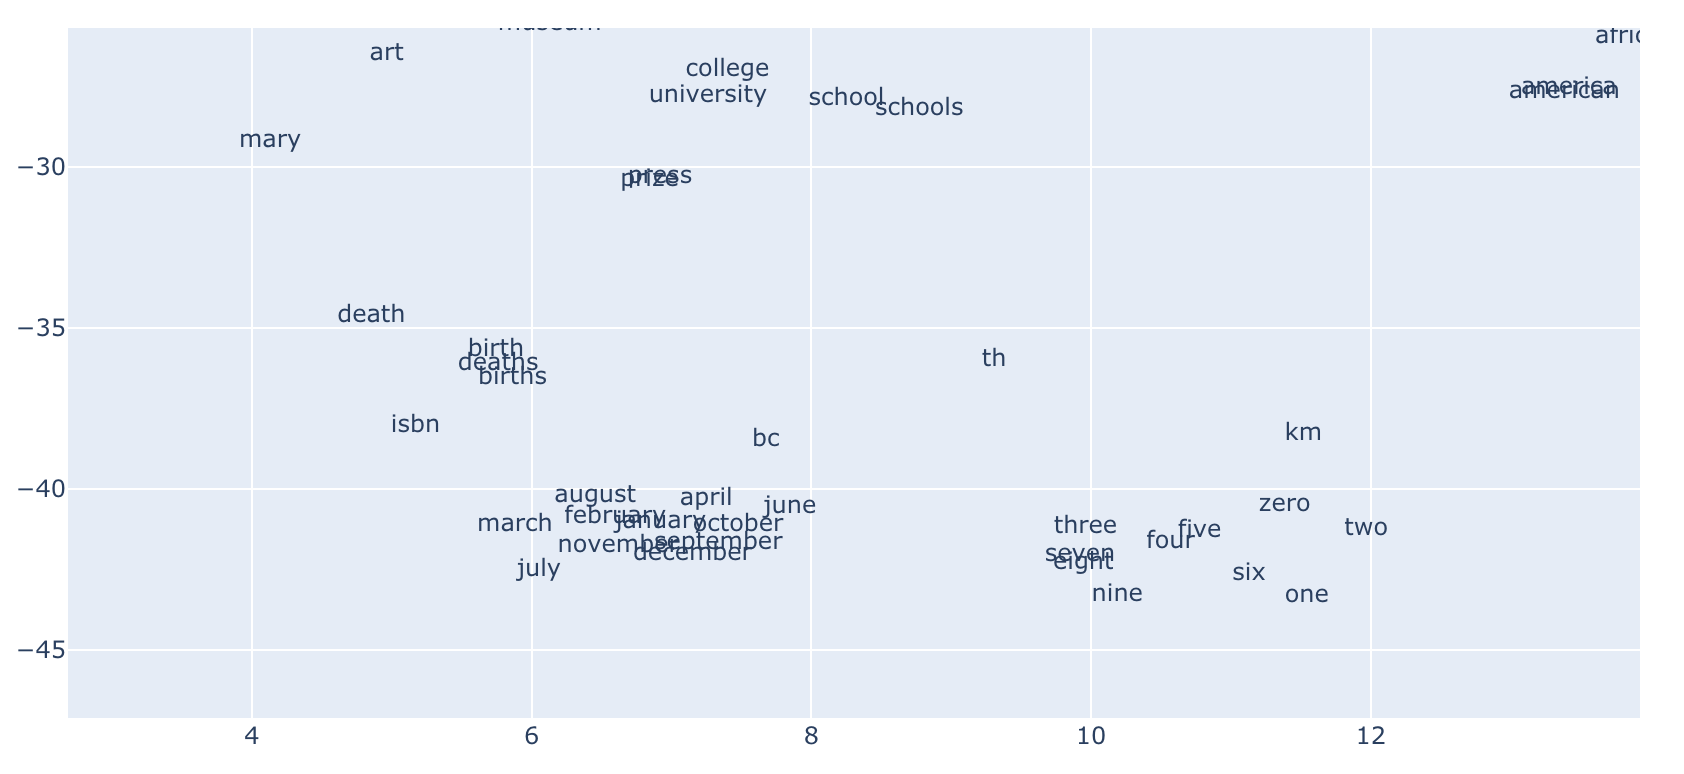
\includegraphics[width=\linewidth]{pictures/fastText_tSNE_screenshot.png}
    \caption{Some of the word vectors from a 100 dimensional fastText embedding trained on a Wikipedia corpus; projected to 2 dimensions using t-SNE.}
    \label{fig:fastText_tSNE}
\end{figure}

Words which are used in similar contexts usually have similar meanings.\footnote{This is not always true, as the words `good' and `bad' demonstrate, more on this below.}
The \emph{distributional hypothesis} states that words which frequently appear in similar contexts have similar meanings.
There is \emph{first-order co-occurence}, also called \emph{syntagmatic association}, if the words are typically nearby each other; for example: `wrote' and `book', `wrote' and `poem'.
We also observe \emph{second order co-occurence}, called \emph{paradigmatic association}, if the words have similar neighbors; for example: `wrote' and `said', `wrote' and `remarked'.

This makes it possible to acquire meaningful representations from unlabeled data -- and there is lots of unlabeled data, e.g., in the form of text from Wikipedia, books, or news headlines.
Thus, we can make both \emph{distributed} and \emph{distributional representations}:
Distributional means that it is based on counts of words in context;
distributed means that the representation is vector based.

The task of finding good word embeddings becomes hard because there are many subtleties in the usage of words in natural language.
Words (or \emph{lemmas}) like `mole' can have multiple meanings, which are its \emph{word senses}; a word which has multiple meanings is \emph{polysemous}.
The embedding should also be able to capture concepts such as \emph{synonyms} (words have the same meaning in many or all contexts) and \emph{antonyms} (the word senses are opposites with respect to one feature of the meaning), \emph{similarity}, \emph{relatedness}, \emph{connotation} or \emph{sentiment}.
There is usually a \emph{super-subordinate} relation (also called \emph{hyperonymy}, \emph{hyponymy} or ``is-a'' relation).
On the other hand, \emph{stop words} like `a', `the', `is', `are', `and' are so commonly used that they carry very little useful information.

There is a big difference between \emph{static} and \emph{contextualized} embeddings:
In a \emph{static embedding} (\Cref{sec:static_word_embeddings}) there is one fixed embedding for each word in the vocabulary.
In a \emph{contextual embedding} (\Cref{sec:contextual_word_embeddings}) the vector we associate to a word is different if it is used in a different context.

We will also talk about how one can try to evaluate the quality of a word embedding.
In \emph{extrinsic evaluation} in a downstream task, we use a word embedding for a specific task and measure whether it increases performance; \emph{intrinsic evaluation} is a harder challenge.

% % % % % % % % % % % % % % % % % % %
\subsection{General References and Links}
\label{sec:general_references}

\begin{itemize}
    \item For a general introduction see the book \cite{jurafsky2009speech}, but take a look at the \href{https://web.stanford.edu/~jurafsky/slp3/}{draft of the 3rd edition}, in particular Chapter 6 on ``Vector Semantics and Embeddings''.
    There are corresponding \href{https://web.stanford.edu/~jurafsky/slp3/slides/6_Vector_Apr18_2021.pdf}{slides} as well.

    \item \cite[Chp.~14]{eisenstein2019introduction} on ``Distributional and Distributed Semantics'';
    draft available \href{https://github.com/jacobeisenstein/gt-nlp-class/blob/master/notes/eisenstein-nlp-notes.pdf}{here}.

    \item \href{https://www.cs.hhu.de/fileadmin/redaktion/Fakultaeten/Mathematisch-Naturwissenschaftliche_Fakultaet/Informatik/Dialog_Systems_and_Machine_Learning/20190705_word_embeddings.pdf}{Michael Heck's slides on the Space of Word Embeddings}.
    
    \item \href{https://lena-voita.github.io/nlp_course}{Lena Voita's NLP Course For You}, in particular the lesson on \href{https://lena-voita.github.io/nlp_course/word_embeddings}{Word Embeddings} and the lesson on \href{https://lena-voita.github.io/nlp_course/seq2seq_and_attention.html}{Sequence to Sequence (seq2seq) and Attention}.
    
    \item \href{https://youtube.com/playlist?list=PL75e0qA87dlG-za8eLI6t0_Pbxafk-cxb}{Rasa Algorithm Whiteboard} YouTube playlist.
    
    \item \href{https://www.youtube.com/c/aicoffeebreak}{AI Coffee Break with Letitia} YouTube channel.
\end{itemize}

% % % % % % % % % % % % % % % %
\subsubsection{Acknowledgments}

The content of this document is based on the seminar ``Word embedding spaces'' run at HHU Düsseldorf in the Summer Term 2022.
I am grateful for the suggestions and feedback collected during the sessions. \\
Sections of this write-up are based on the final reports written by the students:
\begin{itemize}
	\item Nick Rucks: fastText and GloVe
	\item Lukas Rücker: Sequence to Sequence and Recurrent Methods
	\item Benedikt Prusas, Benedikt Jung: Transformers
	\item Thanh Nam Le, Michail Angelos Severino Theoktistou: Masked Language Models and BERT
\end{itemize}

\noindent Thank you to Milica Gašić, Chris Geishauser, Michael Heck for additional input. \\
AI writing assistants such as ChatGPT and GitHub Copilot where used in generating these learning materials. \\

%~~~~~~~~~~~~~~~~~~~~~~~~~~~~~~~~~~~~~~~~~~%
\section{Background and Static Word Embeddings}
\label{sec:static_word_embeddings}
%~~~~~~~~~~~~~~~~~~~~~~~~~~~~~~~~~~~~~~~~~~%


% % % % % % % % % % % % % % % % % % %
\subsection{Frequency based methods}

TODO: Add abstract on frequency based methods

\noindent \textbf{References:}
\begin{itemize}
    \item General references in \Cref{sec:general_references};
    \item Using ``tricks'' from word2vec to improve count-based models \cite{levy-etal-2015-improving};
    \item Skip-gram with negative-sampling (SGNS, see word2vec below) implicitly factorizes the shifted pointwise mutual information (PMI) matrix \cite{NIPS2014_feab05aa}.
\end{itemize}

{
	\color{blue}
	
	Co-occurence counts;
	term-document matrix: each document is represented by a vector of word counts;
	\textbf{t}erm \textbf{f}requency -- \textbf{i}nverse \textbf{d}ocument \textbf{f}requency (tf-idf):
	sparse vectors, words are represented as a simple function of the counts of neighbors;
	\textbf{p}ointwise \textbf{p}ositive \textbf{m}utual \textbf{i}nformation (PPMI):
	$\operatorname{PMI}(w_{1}, w_{2}) = \log \frac{p(w_{1}, w_{2})}{p(w_{1}) \cdot p(w_{2})}$;
	dense versus sparse embeddings;
	Latent semantic analysis:
	singular value decomposition applied to term-document matrix (weighted by log frequency and normalized by entropy);
	cosine similarity.
} % END color blue

% % % % % % % % % % % % % % % % % % %
\subsection{word2vec}

TODO: Add abstract on word2vec

\noindent \textbf{References:}
\begin{itemize}
	\item The original sources are
	\cite{DBLP:journals/corr/abs-1301-3781},
	\cite{DBLP:journals/corr/MikolovSCCD13}.
	\item The survey \cite{DBLP:journals/corr/Rong14} has a detailed explanation of the parameter update equations in word2vec.
    \item \cite{DBLP:journals/corr/abs-1901-09813} try to find a theoretical explanation for these linear relations.
    \item Similarities across languages can be detected in the embeddings \cite{DBLP:journals/corr/MikolovLS13}, which allows constructions of mappings between semantic spaces even without having parallel data \cite{DBLP:journals/corr/abs-1710-04087}.
    \item Such an analysis can lead to ideas for improving the embeddings, as in \cite{DBLP:journals/corr/MuBV17} (they subtract the mean from the word vectors and eliminate top PCA components).
    \item \href{https://gluebenchmark.com/}{General Language Understanding Evaluation (GLUE) benchmark}, \href{https://super.gluebenchmark.com/}{SuperGLUE}
\end{itemize}

{
	\color{blue}
	
	static embedding;
	\textbf{s}kip-\textbf{g}ram with \textbf{n}egative \textbf{s}ampling (SGNS);
	Idea: train a classifier to a prediction task `the word $w$ is likely to show up near the word $c$';
	self-supervision: can use the next word in a corpus of running text as the supervision signal
	\begin{itemize}
		\item get positive examples from taking a target word $w$ and its neighboring context words (have to choose a context window size $L$, these notes \cite{DBLP:journals/corr/Goldberg15c} discuss the effect of the window size).
		\item randomly sample other words to get negative examples (based on the empirical distribution of words, but usually modified to sample less frequent words more often).
		\item train a classifier (for example by logistic regression, i.e.\ the probability score is given as the sigmoid of the dot product) to distinguish the two cases;
		skip-gram makes simplifying assumption that all context words are independent.
		\item the learned weights of the classifier give the embedding of the word $w$:
		target embedding in matrix $W$ and context embedding in matrix $C$.
	\end{itemize}
	Variations of word2vec training methods:
	\begin{itemize}
		\item Skip-Gram:
		predict context words given the central word.
		\item \textbf{C}ontinuous \textbf{B}ag-\textbf{o}f-\textbf{W}ords (CBOW):
		predict the central word from the sum of context words (this sum is called the ``bag of words'').
		\item Simple, but powerful approach:
		Represent a sentence with the average of its word embeddings.
		Hybrid: word embeddings are computed distributionally, and the sentence embedding computed by composition.
	\end{itemize}
	
	Evaluating word embeddings:
	\emph{Intrinsic evaluation} measures how well the word vectors capture meaning, for example by evaluating on word similarity and word analogy tasks;
	\emph{extrinsic evaluation} is performed by looking at the performance of a downstream task.
	Linear structure in the embedding space can be observed from word analogies, such as that the vector of
	\[
	v_{\textup{king}} - v_{\textup{man}} + v_{\textup{woman}} \text{ is close to } v_{\textup{queen}}.
	\]
} % END color blue

% % % % % % % % % % % % % % % % % % %
\subsection{GloVe}

GloVe~\cite{pennington-etal-2014-glove} stands for ``global vectors'', which refers to the fact that the model captures global corpus statistics directly. 
This is similar to most matrix factorization methods but GloVe additionally provides dense vector representations and has a linear substructure in the vector space. 
Therefore, it combines the advantages of global factorization methods and local context window methods. 
On the other hand, it cannot handle OOV words. However, by efficiently training on huge corpora, it can at least decrease the occurrence probability for OOV words. \\

Starting point for learning the GloVe embeddings are the ratios of co-occurrence probabilities
\begin{equation}
	\frac{P_{ik}}{P_{jk}},
\end{equation}
where $P_{ik}$ is the probability that word $k$ appears in the context of word $i$. Further the probability is defined by
\begin{equation}
	P_{ij} = \frac{X_{ij}}{\sum_{k} X_{ik}},
\end{equation}

where $X_{ij}$ is the frequency that word $j$ occurs in the context of word $i$ while $\sum_{k} X_{ik}$ is the sum of co-occurrence frequencies of all words $k$ in the context of word $i$.
The ratios from Equation (2) are able to discriminate relevant from irrelevant words in the corpus. Hence from these ratios, the authors derive a weighted least squares objective to learn the GloVe embeddings, i.e., they optimize
\begin{equation}
	\mathcal{J} = \sum_{i,j = 1}^V f(X_{ij})(w_i^\top\widetilde{w}_j + b_i + \widetilde{b}_j - \log X_{ij})^2
\end{equation}
where $w_i$ and $\widetilde{w}_j$ are the randomly initialized vector representations for the target word $i$ and context word $j$ while $b_i$ and $\tilde{b}_j$ are bias terms that are learned together with the embeddings. The loss imposes that the inner product of the word vectors $w_i^\top\widetilde{w}_j$ should be approximately equal to their log co-occurrence counts $\log X_{ij}$. Hence, GloVe can be viewed as a matrix factorization method. The weighting function $f$ penalizes irrelevant word pairs, either if they are too rare or too frequent. During optimization of $\mathcal{J}$, the authors sample non-zero entries $X_{ij}$ from the co-occurrence matrix $X$. This matrix tabulates how often words co-occur with each other and can be obtained by a single pass through the whole corpus.\\

The GloVe embeddings are successfully evaluated on the word analogy task, validating that the vector space contains linear sub-structures. Moreover, it is demonstrated that GloVe embeddings achieve better results on the word similarity task than embeddings from Word2Vec. In general, GloVe is able to consistently outperform Word2Vec in a similar training setting. Moreover, since it can leverage bigger amounts of data it further provides a better representation for rare words than Word2Vec. Finally, during the extrinsic evaluation the performance on a Named entity recognition (NER) task could be improved using GloVe embeddings as features compared to a CBOW embeddings from Word2Vec.

{
	\color{blue}
		
	static embedding;
	captures global corpus statistics (so it considers global context), based on ratios of probabilities from word-word co-occurrence matrix $X_{ij}$;
	these counts are used to define the loss function, which leads to minimization of a sum of squares
	\begin{equation*}
	    J = \sum_{i, j} \frac{X_{ij}}{X_{\textup{max}}}
	    (w_{i} \widetilde{w_{j}}^{T} - \log X_{ij})^{2}
	\end{equation*}
	$w_{i}$ is the word vector and $\widetilde{w_{j}}$ the context vector;
	can add in a weighting function to penalize rare events and not over-weight frequent events, and add in bias terms for each weight vector;
	does not handle out of vocabulary (OOV) words;
}

\noindent \textbf{References:}
\begin{itemize}
	\item Original source \cite{pennington-etal-2014-glove},
	\href{https://nlp.stanford.edu/projects/glove/}{GloVe project page}.
\end{itemize}

% % % % % % % % % % % % % % % % % % %
\subsection{fastText}

FastText~\cite{DBLP:journals/corr/BojanowskiGJM16} is an extension of the Skip-gram model introduced by \cite{DBLP:journals/corr/MikolovSCCD13} and therefore belongs to the family of local context window methods. In contrast to Skip-gram and Continuous Bag-of-Words (CBOW)~\cite{DBLP:journals/corr/MikolovSCCD13} it is able to embed out-of-vocabulary (OOV) words. Furthermore, by considering character level information it improves the representation for rare and compound words which leads to an increased performance, especially for morphologically rich languages like German or Finnish.\\

FastText computes a bag of constituent $n$-grams $\mathcal{G}_w$ for each word $w$ in the corpus, containing the word itself plus all $n$-grams for a predefined range of $n$. Then, the word representation $\textbf{u}_w$ is the sum of $n$-gram embeddings $\textbf{z}_g$ obtained by a pre-trained Skip-gram model, i.e.,
\begin{equation}
	\textbf{u}_w = \sum_{g \in \mathcal{G}_w} \textbf{z}_g.
\end{equation}
Besides the different representation $\textbf{u}_w$, the training of the objective is adopted from the Word2Vec framework.\\

The authors show in an intrinsic evaluation that the inclusion of character level information enables an improved performance on the word similarity task compared to Word2Vec. This also holds for the syntactic questions of the word analogy task. Moreover, the representations that FastText computes for OOV words always improves the performance on the word similarity task which validates that the representations are reasonable. During further evaluation, the authors showed that the most important $n$-grams in the representation actually correspond to valid morphemes, e.g., prefixes and suffixes. For that, the authors omitted a single $n$-gram from the representation $\textbf{u}_w$ to get a restricted representation $\textbf{u}_{w\setminus g}$. Then, they ranked all $n$-grams by their cosine distance between $\textbf{u}_w$ and $\textbf{u}_{w\setminus g}$, to determine the importance of each $n$-gram for $\textbf{u}_w$. Furthermore, the better usage of subword information enables FastText to obtain better embeddings from smaller datasets than Word2Vec. Additionally, the word representation trained with subword information outperforms plain Skip-gram embeddings on a language modeling task.

{
	\color{blue}
	
	static embedding;
	deals better with unknown words and word sparsity;
	add special boundary symbols < and > to the word,
	example for $n=3$ and the word `where':
	<where> and <wh, whe, her, ere, re>;
	learn skip-gram embedding for each constituent $n$-gram, word is represented by the sum of all the embeddings of the constituent $n$-grams;
} % END color blue

\noindent \textbf{References:}
\begin{itemize}
	\item Original source \cite{DBLP:journals/corr/BojanowskiGJM16}
\end{itemize}


%~~~~~~~~~~~~~~~~~~~~~~~~~~~~~~~~~~~~~~~~~~%
\section{Contextual Word Embeddings}
\label{sec:contextual_word_embeddings}
%~~~~~~~~~~~~~~~~~~~~~~~~~~~~~~~~~~~~~~~~~~%

% % % % % % % % % % % % % % % % % % % % % % % % % % % % % % %
\subsection{Sequence to sequence tasks and Recurrent networks}


\subsubsection{Motivation}

Modeling language using static embeddings like word2vec or Glove, there are a few problems. Different meanings of the same word cannot be accurately captured, as each word has only a single vector embedding. Thus, depending on the training corpus, the embedding will either only capture a single meaning, or the embedding will be the average of different meanings. Furthermore, these embeddings allow for simple arithmetic operation that capture some meaning, but these lack the flexibility to capture the interaction between words that are so essential to language. To tackle more complex tasks like translation we need to rethink language modelling to integrate a source input. One way to do this is by using an Encoder-Decoder architecture \cite{voitseq2seq}. 

\subsubsection{Encoder and Decoder}
The idea of the Encoder-Decoder architecture, is that the Encoder takes an input and produces a latent representation. The Decoder uses this representation to (re-)create information. More specifically, using translation as an example (throughout this abstract) it looks like this: The Decoder uses the given representation of a source sentence to create a translation. For translations recurrent neural networks (RNNs) have proven to be effective implementation for this.

\subsubsection{Recurrent Neural Networks}
A RNN is a neural network that is getting repeated throughout time, and at each time step $t$ there can be a new input and output. The crux because RNNs are eligible for NLP task, is that the hidden layer at time step $t-1$ influences the hidden layer at time step $t$. Thus, the problem of lacking the ability to capture language dependencies between words is being tackled. A RNN can then be used both as the Encoder and as the Decoder. RNNs in their basic form, can run into problems during model training because of vanishing or exploding gradients  \cite{sutskever2014sequence}. Furthermore, the information propagation is not ideal for longer sequences and performance suffers. To address this a commonly used modification is using a Long Short-Term Memory (LSTM) RNN. 

\subsubsection{Long Short-Term Memory}
A LSTM is a different kind of RNN, where the internal structure of each reoccurring unit is different. Besides the hidden state, there is an additional cell state. This cell state gets passed through each unit, with little interference. It helps to keep the gradient in appropriate ranges as well as transfer information through many units \cite{karpathyRNN}. With these LSTMs Peters et al. designed a model named Embeddings from Language Models (ELMo), to tackle the problem of finding embeddings for polysemic words.

\subsubsection{Embeddings from Language Models (ELMo)}
ELMo produces a different embedding for each word dependent on the sentence it is used in. This is implemented as a multi-layered bidirectional LSTM. Using an LSTM for each direction ensures to capture information of the entire input sequence. The model then combines the hidden state representation of both LSTMs by concatenating them, and them adds up the concatenated states of each layer up with a task-specific weighting \cite{DBLP:conf/naacl/PetersNIGCLZ18}.  The embeddings created by ELMo have the potential to improve the language understanding of many NLP models. Still, using a single vector representation for an entire source sentence is bound to fail at capturing all information. 
To reduce this dependency Bahdanau et al. added the concept of \emph{attention}.
\index{attention}

\subsubsection{Attention}

The idea behind attention is that the model learns to take in more specific information from the single source inputs. 
This can be implemented with a context vector. 
A context vector is the result of calculating attentions scores between a single hidden state of the decoder and all encoder states. 
Using a softmax function, these attention scores can be turned into probabilities or weights. 
Summing up each encoder state weighted by its softmax value, we calculate the context vector \cite{DBLP:journals/corr/BahdanauCB14}.
The decoder at each time step uses this context and is not solely dependent on the single representation from the Encoder. 
If implemented with an appropriate attention score, the whole process is differentiable and can be learned task-specific by the model.

{
	\color{blue}
	
	{E}mbeddings from \textbf{L}anguage \textbf{Mo}dels (ELMo):
	The ElMo architecture is based on earlier ideas using Recurrent Neural Nets (RNNs) to model sequences, such as sentences in natural language.
	ElMo produces deep contextualized word representations, which are learned functions of internal states of a deep bidirectional language model with Long short-term memory (LSTM) units.
	ELMo embeddings are context-sensitive, i.e.\ each token representation is a function of the entire input sentence.
	Here lower layers appear to capture syntactics, while higher layers capture semantics.
	ELMo is unsupervised, can handle OOV, but is not truly bidirectional.
} % END color blue

\noindent \textbf{References:}
\begin{itemize}
	\item \textbf{Original ELMo research article:} `Deep Contextualized Word Representations' \cite{DBLP:journals/corr/abs-1802-05365}.
	\item The concept of attention, which lets a model focus on different parts of the input while processing a sequence, was introduced in \cite{garg-etal-2019-jointly}.
	\item Lecture notes: \href{https://lena-voita.github.io/nlp_course/seq2seq_and_attention.html}{Sequence to Sequence (seq2seq) and Attention}
\end{itemize}

% % % % % % % % % % % % % % % % % % % % % % % % % % % % % % %
\subsection{Transformers}

The authors in \cite{DBLP:journals/corr/VaswaniSPUJGKP17} introduce a neural network architecture for the task of machine translation without any recurrence. 
This resolves the problems of recurrent neural networks such as weak long range dependencies, training instability and scale-ability.

We can view a transformer as a ``sequence to sequence'' model and differentiate between stacked encoder and decoder blocks.

Embeddings get contextualized throughout multiple encoder blocks.
The information flows through the attention mechanism and is processed by basic feed forward layers. 

Ultimately, the blocks can be broken down to matrix operations and the attention formulation is derived from a database analogy \cite{pmlr-v139-schlag21a}.

\noindent \textbf{References:}
\begin{itemize}
	\item \textbf{Original research article:} `Attention is all you need' \cite{DBLP:journals/corr/VaswaniSPUJGKP17}.
	\item Blog post:
	\href{https://jalammar.github.io/visualizing-neural-machine-translation-mechanics-of-seq2seq-models-with-attention/}{'Visualizing A Neural Machine Translation Model (Mechanics of Seq2seq Models With Attention)'}
	\item Blog post:
	\href{https://jalammar.github.io/illustrated-transformer/}{'The Illustrated Transformer'}
	\item Blog post:
	\href{http://peterbloem.nl/blog/transformers}{'Transformers from scratch'}
	\item PyTorch implementation \href{https://nlp.seas.harvard.edu/2018/04/03/attention.html}{'The Annotated Transformer'}
	\item Vision transformers \cite{dosovitskiy2021an}
	\item Visualizations of attention maps:
	\href{https://github.com/jessevig/bertviz}{BertViz}
\end{itemize}

{
	\color{blue}
	
	Encoder and decoder block; self-attention mechanism; query, key and value matrices; multi-head attention (combining multiple self-attention mechanisms); positional embeddings; autoregressive models: predict the next token in a sequence, for this we have to mask the self-attention in the decoder block so that the model can only attend to tokens in the preceding sequence.
	The original transformer model was trained on machine translation, which is a sequence to sequence task.
} % END color blue


% % % % % % % % % % % % % % % % % % % % % % % % % % % % % % %
\subsection{Masked Language Models and BERT}

% % % %
\subsubsection{Introduction}

BERT (\textbf{B}i-directional \textbf{E}ncoder \textbf{R}epresentations from \textbf{T}ransformers) follows the Transformer architecture \cite{DBLP:journals/corr/VaswaniSPUJGKP17}; more concretely the encoder part of it. 
BERT allows tokens to attend both previous and posterior tokens. 
This is the main advantage setting BERT apart from previous language representation models. 
Two BERT versions are trained, BERT-Base to be compared with the Open AI's GPT model and BERT-Large with more blocks, attention heads, and a larger hidden dimension.

% % % % 
\subsubsection{Model Input}

As input, BERT accepts either single or a pair of sentences, which are simply concatenated with a special token [SEP] in between.
To enable down-stream tasks, there is also a classification token [CLS] at the beginning.
To further distinguish the tokens belonging to each sentence, a third segment embedding is used, besides the usual token and positional embeddings known from the standard transformer. 
Tokenization is generated via WordPiece \cite{wu2016google}. 
WordPiece uses a 30k token vocabulary, each word is searched in this corpus and if it does not exist it will be decomposed into constituent pieces. 
This input embedding is static at first but will become contextualized after going through the model.

% % % %
\subsubsection {BERT Architecture}

BERT uses a multi-layer bidirectional transformer encoder. 
This encoder is based on the original transformer encoder. 
Each BERT layer contains two normalization layers, a feed forward layer and a multi-head attention layer. 
The major difference is that BERT uses bidirectional self-attention, words can see them selves, there is no constrain, while the GPT transformer uses constrained self-attention where every token can only attend to the context to its left. 
BERT comes in two sizes:
BERT Base has 12 layers, a hidden size of 768, 12 self-attention heads and 110M parameters to train. 
BERT Base has the same model size as GPT so their performances are comparable. 
BERT Large has 24 layers, a hidden size of 1024, 16 self-attention heads and a total of 340M to train. 
BERT Large is to achieve better results on benchmarks stated in the paper.

% % % % 
\subsubsection{Pre-training and Fine-tuning}

BERT is pre-trained using BooksCorpus and the English Wikipedia, via two unsupervised tasks as follows:

\begin{enumerate}
	\item Masked Language Model (MLM). 
	To avoid mappings between input-output due to a bidirectional context where words can see themselves, 15 percent of the tokens are randomly masked. 
	The masked tokens are then predicted, as the final hidden vectors corresponding to them are fed into a softmax over the vocabulary. 
	To mitigate a mismatch between pre-training and fine-tuning as there is no [MASK] token during fine-tuning, only 80 percent of the chosen tokens are replaced by [MASK]; 10 percent are replaced by a random token, and the remaining 10 percent are left unchanged, as illustrated below:
	\begin{itemize}
		\item my cat is hungry $\leadsto$ my cat is [MASK]
		\item my cat is hungry $\leadsto$ my cat is president
		\item my cat is hungry $\leadsto$ my cat is hungry
	\end{itemize}
	
	\item Next-Sentence-Prediction (NSP).
	We want to predict if sentence B is the actual sentence that proceeds sentence A or not. 
	This task is beneficial for downstream tasks that require understanding the relationship between sentences, such as question-answering.
	To learn this relationship between sentences, a binary classification task is used where sentence B is 50 percent of the time the one that follows sentence A (label = \textit{IsNext}), and 50 percent of the time is chosen randomly (label = \textit{NotIsNext}). 
	Here are two examples.
	\begin{itemize}
		\item [CLS] The man went to [MASK] store [SEP] He bought a gallon [MASK] milk [SEP] $\leadsto$ \textit{IsNext}
		\item [CLS] The man went to [MASK] store [SEP] Penguins [MASK] flightless birds [SEP] $\leadsto$ \textit{NotIsNext}
	\end{itemize}
\end{enumerate}

Fine-tuning is done by initializing the model with the pre-trained weights to adapt for specific tasks. 
During this process the pre-trained weights change slightly and the tasks specific weights are learned.
In the paper, BERT is fine-tuned for 12 different NLP tasks.
The BERT Large model is shown to be the best-performing system across the multi-task GLUE benchmark, the SQuAD benchmark (both version 1.1 and 2.0) as well as the SWAG benchmark.

% % % %
\subsubsection{Conclusion}

The authors show that Transformers continue to be state-of-the-art in many NLP tasks. 
They exhibit the benefits of using a true bidirectional structure based on a MLM, which allows to solve more downstream tasks. 
They also show how BERT can be trained relative faster and in a more efficient way by using the self-attention mechanism from transformers that use parallel training instead of traditional LSTMs that use sequential training.

\noindent \textbf{References:}
\begin{itemize}
	\item Original research article:  \cite{DBLP:journals/corr/abs-1810-04805}
	\item \href{https://lena-voita.github.io/nlp_course/transfer_learning.html}{(Introduction to) Transfer Learning} in the NLP for you course.
	\item \cite{clark-etal-2019-bert} analyze the role of the different attention heads in the trained BERT model.
	\item A \textbf{Ro}bustly \textbf{O}ptimized \textbf{BERT} Pretraining \textbf{A}pproach (RoBERTa):
	The authors observe that BERT was significantly under-trained, and update the model \cite{DBLP:journals/corr/abs-1907-11692}.
	\item GPT for language generation.
\end{itemize}

{
	\color{blue}
	
	The objective of the BERT model is a \emph{Masked language modeling task}, in which we randomly mask words in the training text and try to predict the masked words from their context.
	Additionally, the model is trained on a \emph{next sentence prediction} task.
	For the input embedding: WordPiece tokenization;
	special \texttt{[CLS]} token for the representation of the entire input sequence.
} % END color blue


% % % % % % % % % % % % % % % % % % %
\subsection{Sentence Embeddings}

TODO: Add abstract for Sentence Embeddings


\noindent \textbf{References:}
\begin{itemize}
	\item Sentence-BERT: \cite{DBLP:journals/corr/abs-1908-10084} and \href{https://www.sbert.net/}{SentenceTransformers}
	find an embedding on the sentence level so that semantically similar sentences are close in the embeddings space;
	adds a pooling operation to the output of BERT or RoBERTa to derive a fixed sized sentence embedding;
	siamese and triplet network structures.
	\item TransEncoder: For pairwise comparison of sentences, \cite{DBLP:journals/corr/abs-2109-13059} alternate between a bi-encoder (which produces fixed-dimensional sentence embeddings) and a cross-encoder (which has attention heads that span the complete sequence of both sentences), so that they learn from each other to train an unsupervised sentence representation model.
	\item SimCSE \cite{DBLP:journals/corr/abs-2104-08821}: Uses contrastive learning to improve sentence embeddings, where the positive pairs are created by adding dropout in the encoder as the noise.
	\item Dialog utterance embeddings via contrastive learning \cite{https://doi.org/10.48550/arxiv.2205.13568}
	\item Video: \href{https://youtu.be/O3xbVmpdJwU}{Transformer Neural Networks - an Overview!}
\end{itemize}

{
	\color{blue}
	
	\emph{Contrastive learning} (pull semantically close neighbors together and push apart non-neighbors) for sentence embeddings:
} % END color blue


% % % % % % % % % % % % % % % % % % %
\subsection{Multi-modal Embeddings}

\begin{itemize}
	\item Joint text and image space:
	\cite{DBLP:journals/corr/abs-2111-07180}
	
	\item \href{https://openai.com/blog/clip/}{CLIP: Connecting Text and Images};
	\cite{radford2021learning}
\end{itemize}



TODO: Add more references

%~~~~~~~~~~~~~~~~~~~~~~~~~~~~~~~~~~~~~~~~~~%
\section{Structure in Word Embeddings}
%~~~~~~~~~~~~~~~~~~~~~~~~~~~~~~~~~~~~~~~~~~%

% % % % % % % % % % % % % % % % % % % % % % % %
\subsection{Sentiment specific word embeddings}

TODO Add abstract on sentiment in word embeddings

\noindent \textbf{References:}
\begin{itemize}
	\item Using sentiment aware word embeddings for emotion classification \cite{sentiment-aware-word-embedding-emotion-2019};
	\item TweetEval dataset, which includes emotion recognition and sentiment analysis tasks \cite{barbieri-etal-2020-tweeteval}, the authors released their \href{https://huggingface.co/cardiffnlp/twitter-roberta-base-sentiment}{pre-trained RoBERTa models};
	\item German sentiment classification with using fastText and BERT embeddings \cite{guhr-etal-2020-training};
	\item EmoWOZ \cite{DBLP:journals/corr/abs-2109-04919} is a task-oriented dialogue dataset annotated with emotions.
\end{itemize}

{
	\color{blue}
	
	\emph{Sentiment} is a positive or negative evaluation, and we can enhance our \emph{semantic} specific word embeddings with \emph{sentiment} \cite{yu-etal-2017-refining}.
	Words with similar vector representations can have an opposite sentiment polarity (e.g., `good' vs `bad' or `happy' vs `sad').
	To capture this in the embedding one can add a post-processing step to adapt the pre-trained vectors to sentiment applications,
	where we move the word closer to a set of both semantically and sentimentally similar nearest neighbors (i.e., those with the same polarity) and further away from sentimentally dissimilar neighbors (i.e., those with an opposite polarity).
} % END color blue



% % % % % % % % % % % % % % % % % % % % % % % %
\subsection{Bias in Word Embeddings}

\noindent \textbf{References:}
\begin{itemize}
	\item Iterative nullspace projection to debias word embeddings \cite{ravfogel-etal-2020-null};
	\item Visualizations of bias mitigation techniques \cite{DBLP:journals/corr/abs-2104-02797},
	their \href{https://github.com/tdavislab/verb}{code} for creating interactive demos is available online;
	\item Gender bias in the contextualized embeddings from ElMo \cite{zhao-etal-2019-gender};
	\item Bias in BERT embeddings \cite{kurita-etal-2019-measuring};
	\item Debiasing contextualized embeddings \cite{kaneko-bollegala-2021-debiasing}.
\end{itemize}

{
	\color{blue}
	
	A desirable association could be ``a man to a woman is as a king to a queen'', whereas an undesirable association is ``a man to a woman is as a physician to a nurse''.
	Unfortunately, it appears that word embeddings trained on a corpus of text extracted from books and websites tend to incorporate and amplify the biases contained in our language.
	When such biased embeddings are used for downstream tasks, this can lead to bias amplification.
	To investigate gender bias systematically, \cite{DBLP:journals/corr/BolukbasiCZSK16a} take a seed pair $(v_\textup{he}, v_\textup{she})$ and find other pairs of word vectors which have a difference similar to the seed vector.
	They also provide methods for debiasing the embedding, but they argue that bias ultimately appears to come from the training data.
} % END color blue

% % % % % % % % % % % % % % % % % % % % % % % %
\subsection{Multilingual word embeddings}

We want to use a shared embedding space for words across two or more languages, so that words from different languages with different meanings are close in the cross-lingual embedding space;
the hope is that this can improve performance because the model can acquire and transfer knowledge from other languages;
also look at the references from the `Geometry of the word embedding space'-topic, in particular \cite{DBLP:journals/corr/abs-1710-04087} where they aligned embeddings without having parallel data.

\textbf{Further references:}
\begin{itemize}
	\item \href{https://github.com/facebookresearch/MUSE}{MUSE} is an implementation of both supervised and unsupervised multilingual word embeddings with fastText
	\item \cite{DBLP:journals/corr/abs-1808-08933} train unsupervised MWEs;
	\item \cite{DBLP:journals/corr/abs-2007-01852} build language-agnostic BERT Sentence Embedding
    \item Video: \href{https://youtu.be/7tAWk_Coj-s}{Language Agnostic BERT}
    \item Please also take a look at the document in the appendix with further references on multilingual transformer architectures.
\end{itemize}

% % % % % % % % % % % % % % % % % % % % % % % % % % % % %
\subsection{Applications of Word Embeddings in Dialog Systems}

Components of a dialogue system:
\begin{itemize}
	\item Natural Language Understanding (NLU)
	\item Dialogue State Tracking (DST)
	\item Policy
	\item Natural Language Generation (NLG)
\end{itemize}

\textcolor{red}{TODO}


% % % % % %
\subsubsection{Aligning Language Models}

\begin{itemize}
	\item InstructGPT  \cite{ouyang2022training}
	\item Sparrow
	\item ChatGPT
\end{itemize}

\textcolor{red}{TODO}

%~~~~~~~~~~~~~~~~~~~~~~~~~~~~~~~~~~~~~~~~~~~~~~~~%
\section{Topological Data Analysis and Word Embeddings}
%~~~~~~~~~~~~~~~~~~~~~~~~~~~~~~~~~~~~~~~~~~~~~~~~%

% % % % % % % % % % % % % % % % % % % % % % % % % % % % %
\subsection{Geometry of the word embedding space}

\textcolor{red}{TODO: Edit this section}

\cite{mimno-thompson-2017-strange} find that in skip-gram with negative sampling the word vectors all point in roughly the same direction, i.e.\ lie in a narrow cone (this is sometimes called \emph{anisotropy}, the opposite of this is \emph{isotropy} where the vectors are directionally uniform);
the context vectors point in the other direction (have negative dot product with the mean of the word vectors),
in contrast to this for GloVe the word and context vectors point in the same direction;


\noindent \textbf{References:}
\begin{itemize}
	\item Anisotropy can also be studied in contextualized word embeddings, see \cite{ethayarajh-2019-contextual}, or for sentence embeeddings \cite{li-etal-2020-sentence}
	\item \cite{nakashole-flauger-2018-characterizing} observe that mappings between semantic spaces usually are only locally linear, and not globally linear;
	\item Method for finding words which are used differently in two text corpora:
	train embedding on each corpus, find a (e.g.\ linearly via orthogonal Procrustes) mapping between the embedding spaces, then words which do not match well under this mapping appear to have different meanings.
	Using historical texts, one can see how the meaning changes through time \cite{hamilton-etal-2016-diachronic};
	\item Different method:
	again train embeddings on two corpora separately, then for each word find the closest vectors in each embedding space, if these differ a lot the embeddings are different \cite{gonen-etal-2020-simple}.
\end{itemize}


% % % % % % % % % % % % % % % % % % % % % % % % % % % % %
\subsection{Embeddings in Curved Geometries}

 Instead of embedding data into an Euclidean vector space, we can associate it to points in a more general ambient manifold.

\textcolor{red}{TODO} 
\begin{itemize}
	\item Manifolds
	\item Geodesics
	\item Riemannian optimization
\end{itemize}

% % % % % %
\subsubsection{Positively Curved Spaces: Spherical Embeddings}

Spherical Word Embeddings \cite{Meng2019SphericalTE}



% % % % % %
\subsubsection{Negatively Curved Spaces: Hyperbolic Embeddings}

For example, we can use so-called \emph{negatively curved spaces}, which leads to \emph{hyperbolic embeddings}.
The geometry of these spaces allows a more efficient representation of tree-like structures and hierarchies, as was observed in \cite{DBLP:journals/corr/NickelK17}
See also this \href{https://bjlkeng.github.io/posts/hyperbolic-geometry-and-poincare-embeddings/}{blog post} discussing the paper, and \href{https://rare-technologies.com/implementing-poincare-embeddings/}{this blog post} with implementation details.
In our case, where we associate words to points in a hyperbolic space, these are called \emph{hyperbolic word embeddings} (which can be constructed e.g.\ with Poincar{\'e} GloVe \cite{DBLP:journals/corr/abs-1810-06546}).
Further references include an earlier paper on hyperbolic text embeddings \cite{DBLP:journals/corr/abs-1806-04313},
these in turn were inspired by hyperbolic image embeddings \cite{DBLP:journals/corr/abs-1904-02239}.
There is also a proposed hyperbolic version of fastText \cite{zhu-etal-2020-hypertext}.
One can also `probe' the contextualized embeddings of a BERT model by mapping into a hyperbolic space \cite{DBLP:journals/corr/abs-2104-03869}, and analyzing the structure of the projected data.

\textcolor{red}{TODO}


% % % % % % % % % % % % % % % % % % % % % % % % % % % % %
\subsection{Manifold Hypothesis and Singularities}

\textcolor{red}{TODO}

% % % % % %
\subsubsection{Topological Polysemy and singularities in word embeddings}

The paper \cite{jakubowski2020topology} studies singular points in a fixed word embedding trained via fastText.
They find that the dimension of the zeroth local homology group of a punctured neighborhood of a word correlates with the number of different meanings of a polysemous word.

\textcolor{red}{TODO}

There have been two main developments in Topological Data Analysis (TDA), which might lead to further interesting application of TDA to word embeddings in the future:
\begin{itemize}
        \item \emph{Persistent homology} is a description of the topological features of a space at various scales.
        Usually the data comes with a \emph{filtration}, and we compute the homology of the pieces which assemble into a \emph{persistence module}.
        These can be encoded into a \emph{bar-code}, which then is used in further machine learning pipelines.
        For example \cite{reinauer2021persformer} develop a Transformer model which takes persistence diagrams as input. 
        
        \item The MAPPER algorithm is a projection technique which also uses clustering to capture more of the global features of the dataset.
        An interesting projection choice is $t$-Stochastic Neighborhood Embedding ($t$-SNE, \cite{JMLR:v9:vandermaaten08a}).
\end{itemize}

Here are some general references for background reading on Topological Data Analysis:
\begin{itemize}
    \item \cite{murugan2019introduction}: Survey paper with an introduction to ``Topological Data Analysis for Physicists''.
    \item \cite{dey2021computational}: Book (draft) on Topological Data Analysis.
    \item Vidit Nanda's \href{http://people.maths.ox.ac.uk/nanda/cat/TDANotes.pdf}{Computational Algebraic Topology Notes}.
\end{itemize}

\newpage
% % % % % % % % % %
% References
\printbibliography
% % % % % % % % % %

\end{document}
%%%%%%%%%%%%%%%%%%%%%%%%%%%%%%%%
%%%%%%%%%%%%%%%%%%%%%%%%%%%%%%%%